% ======================================================================
%  Computer Physics Communications (CPC) manuscript
%  Official format
% ======================================================================
\documentclass[final,1p,times]{elsarticle}
\usepackage[utf8]{inputenc}
\usepackage{booktabs}
\usepackage{amsmath}
\usepackage{amssymb}
\usepackage{hyperref}
\usepackage{listings}
\usepackage{algorithm}
\usepackage{algpseudocode}
\usepackage{xcolor}
\usepackage{graphicx}
\usepackage{longtable}
\usepackage{rotating} % For landscape sideways figures
\usepackage{tikz}
% Replaced LuaTeX-only libraries with standard pdflatex compatible ones
\usetikzlibrary{positioning,arrows.meta,fit,trees}

\hypersetup{
  colorlinks=true,
  linkcolor=blue,
  citecolor=blue,
  urlcolor=blue
}

\lstset{
  basicstyle=\ttfamily\small,
  breaklines=true,
  frame=single,
  columns=fullflexible,
  keywordstyle=\color{blue},
  commentstyle=\color{gray},
  stringstyle=\color{teal}
}

\newenvironment{programsummary}{%
\section*{Program Summary}
\begin{description}
\setlength{\itemsep}{0.2em}
}{%
\end{description}
}

\journal{Computer Physics Communications}

\begin{document}

% ======================================================================
%  Title and Authors
% ======================================================================
\begin{frontmatter}

\title{trj\_analysis: GPU-accelerated analysis of large LAMMPS NetCDF trajectories}

% -----------------------------
% Authors with affiliations
% -----------------------------
\author[1,2]{Enrique Lomba\corref{cor1}}
\ead{enrique.lomba@csic.es}

\author[3]{Rodrigo Lomba-Moreno}

\author[1]{Antonio D\'{\i}az-Pozuelo\corref{cor2}}
\ead{adiaz@iqf.csic.es}

% -----------------------------
% Corresponding authors
% -----------------------------
\cortext[cor1]{Co-corresponding author.}
\cortext[cor2]{Corresponding author.}

% -----------------------------
% Affiliations (numeric)
% -----------------------------
\address[1]{Instituto de Qu\'{i}mica F\'{i}sica Blas Cabrera, CSIC, Madrid, Spain}
\address[2]{Grupo NAFOMAT, Facultade de Física, Universidade de Santiago de Compostela, Santiago de Compostela, Spain}
\address[3]{ETSI Ingeniería Informática, Campus de Montegancedo, Universidad Politécnica de Madrid, Madrid, Spain}

\begin{abstract}
We present \texttt{trj\_analysis}, a high-performance trajectory analysis toolkit for molecular dynamics simulations generated with LAMMPS and stored in NetCDF format. The code combines modern Fortran (F90/F2008) with GPU acceleration via NVIDIA compilers (\texttt{nvfortran} and \texttt{nvcc}). The package implements a range of structural and dynamical observables, optimized for large systems and long trajectories. A modular architecture supports extensibility, offering comprehensive tools for density-based cluster identification, charge-charge correlations, and confinement-resolved structural profiles. Performance benchmarks illustrate significant speedups using GPU acceleration. We include validation against reference data and provide examples and documentation to support reproducible workflows.
\end{abstract}

\begin{keyword}
Molecular dynamics \sep Trajectory analysis \sep LAMMPS \sep NetCDF \sep GPU acceleration \sep CUDA Fortran
\end{keyword}

\end{frontmatter}

% ======================================================================
%  Program Summary
% ======================================================================
\begin{programsummary}

\item[Program Title:] trj\_analysis
\item[CPC Library link:] (to be assigned)
\item[Developer's repository link:] \url{https://github.com/elomba/trj_analysis}
\item[Licensing provisions:] GPL V3.0
\item[Programming language:] Fortran (F90/F2008), C++
\item[External routines/libraries:] NetCDF, FFTW3, CUDA toolkit
\item[Nature of problem:]
Analysis of large LAMMPS trajectories stored in NetCDF format\cite{Rew1990} can be time-consuming for high-resolution structural and dynamical quantities, especially when cluster analysis is also required. Efficient, scalable tools are needed to process data for scientific insight.
\item[Solution method:]
The program \texttt{trj\_analysis} provides a modular GPU-accelerated framework for trajectory post-processing based on NetCDF trajectory files generated by LAMMPS. The code implements parallel algorithms for radial distribution functions, static and dynamic structure factors, cluster identification, confinement-resolved density profiles, time correlation functions, and Steinhardt bond--orientational order parameters. Independent analysis modules are activated through a structured namelist input interface, allowing flexible workflows adapted to heterogeneous systems and large datasets.
\item[Restrictions:]
The program supports both single-component and multi-component systems
in two and three spatial dimensions. Confinement analysis applies to
slit-pore geometries along any Cartesian axis ($x$, $y$, or $z$,
configured via the \texttt{idir} parameter) in 3D systems, with coordinates
automatically remapped upon trajectory input to the internal canonical slit
orientation. Input trajectories must be provided in NetCDF format. GPU acceleration
requires NVIDIA hardware and corresponding toolchains. The code
assumes orthogonal simulation cells and a constant number of
particles. Currently only \texttt{real}, \texttt{metal}, and
\texttt{lj} units are supported. This code produces atom-oriented
observables, molecular properties are not computed at this stage, but
an analysis of topology files is provided to generate information on
molecular species present in the simulation sample, and to perform a proper calculation of
degrees of freedom in systems with rigid fragments. 
\item[Additional comments:]
Examples, validation routines and pre- and postprocessing tools are distributed with the software. \textbf{Running time:} Execution time depends on system size, trajectory length, and selected analysis modules. Typical runs for trajectories containing $10^4$--$10^5$ particles and $10^3$ configurations complete within minutes on a modern GPU-enabled workstation.
\end{programsummary}

% ======================================================================
%  Main Sections
% ======================================================================

\section{Introduction}

Molecular dynamics (MD) simulation is a cornerstone of computational studies in condensed matter, soft matter, and biophysics. State-of-the-art simulation packages such as LAMMPS\cite{Thompson2021} can generate trajectories that span millions of particles and millions of time steps, producing datasets whose analysis alone poses significant computational challenges. While MD engines provide efficient integration and sampling, post-processing tools must be equally robust to support modern workflows.

\texttt{trj\_analysis} addresses this issue by offering a high-performance, modular trajectory analysis toolkit for LAMMPS NetCDF dumps\cite{Rew1990}. It supports GPU acceleration to reduce the wall-clock time for computationally intensive routines and provides a suite of observables commonly required in physics and materials science studies. The code is implemented in modern Fortran and C++, and it is openly available under a GPL V3.0 license.

It is worth noticing that several general-purpose trajectory analysis frameworks are available for molecular dynamics simulations. Among the most widely used are \texttt{MDAnalysis}~\cite{MDAnalysis2011,MDAnalysis2016} and \texttt{MDTraj}~\cite{MDTraj2015}, which provide flexible Python-based environments supporting multiple trajectory formats and a broad range of structural observables. These packages are particularly well suited for biomolecular simulations and interactive analysis workflows, but their reliance on interpreted scripting layers and in-memory trajectory representations can limit performance when processing very large particle-based datasets.

For soft-matter and particle-based simulations, the \texttt{freud}
library~\cite{freud2020} offers efficient implementations of neighbor
finding, structural correlations, clustering tools, and
bond-orientational order parameters through a C++ backend with Python
bindings. These capabilities make it a widely used platform for
structural characterization in simulations performed with packages
such as HOOMD-blue \cite{Anderson2020} and LAMMPS. However, its execution model remains primarily CPU-based and is typically integrated into Python workflows rather than standalone high-throughput analysis pipelines.

Compiled trajectory-analysis toolkits such as \texttt{LOOS}~\cite{LOOS2012} and \texttt{Pteros}~\cite{Pteros2019} provide efficient C++ interfaces for trajectory manipulation and structural analysis. While these packages offer improved performance compared with interpreted environments, they do not currently include GPU-accelerated implementations of histogram-based observables or density-based clustering algorithms tailored for large-scale particle simulations. Visualization-oriented environments such as \texttt{OVITO}~\cite{OVITO2025} provide advanced structural characterization tools, including common-neighbor analysis and bond-orientational order parameters, together with scripting interfaces for automated workflows. These tools are primarily designed for interactive inspection and post-processing rather than high-throughput batch evaluation of long trajectories.

In contrast to these packages, \texttt{trj\_analysis} is specifically designed for scalable post-processing of large LAMMPS trajectories stored in NetCDF format. The combination of compiled Fortran/C++ kernels with GPU acceleration enables efficient evaluation of histogram-based structural observables, bond-orientational order parameters, and density-based cluster identification for systems containing hundreds of thousands of particles over long simulation times within a unified command-line workflow.

\section{Software Design and Implementation}

\subsection{Objectives}

The primary design goals are:
\begin{itemize}
  \item Efficient input of NetCDF trajectory files.
  \item Scalable computation of structural and dynamical observables.
  \item Modular separation of I/O, data structures, and analysis kernels.
  \item GPU acceleration for performance-critical operations.
\end{itemize}

\subsection{Architecture}

The software consists of:
\begin{itemize}
  \item A core I/O layer for reading NetCDF trajectories.
  \item A data model representing per-frame particle data and simulation metadata.
  \item Analysis modules implementing specific observables.
  \item Backend kernels for CPU and GPU execution.
\end{itemize}

Fortran (F90/F2008) is used for the main application logic due to its
strong support for numerical arrays, while C++ provides interface to
CUDA Thrust library. GPU acceleration is enabled through NVIDIA's
\texttt{nvfortran} and \texttt{nvcc} compilers which incorporate the
required CUDA language extension to both Fortran and C++. 


% ======================================================
\section{Analysis workflow}

The analysis pipeline implemented in \texttt{trj\_analysis} is
illustrated in Fig.~\ref{fig:workflow}. If needed, simulation trajectories generated with LAMMPS in the standard text-based dump format can be preprocessed using utilities included in the \texttt{tools} directory and transformed to the appropriate NetCDF format\cite{Rew1990} before being analysed by the modular routines that compute structural, cluster and dynamical observables.

\begin{figure}[htbp]
\centering
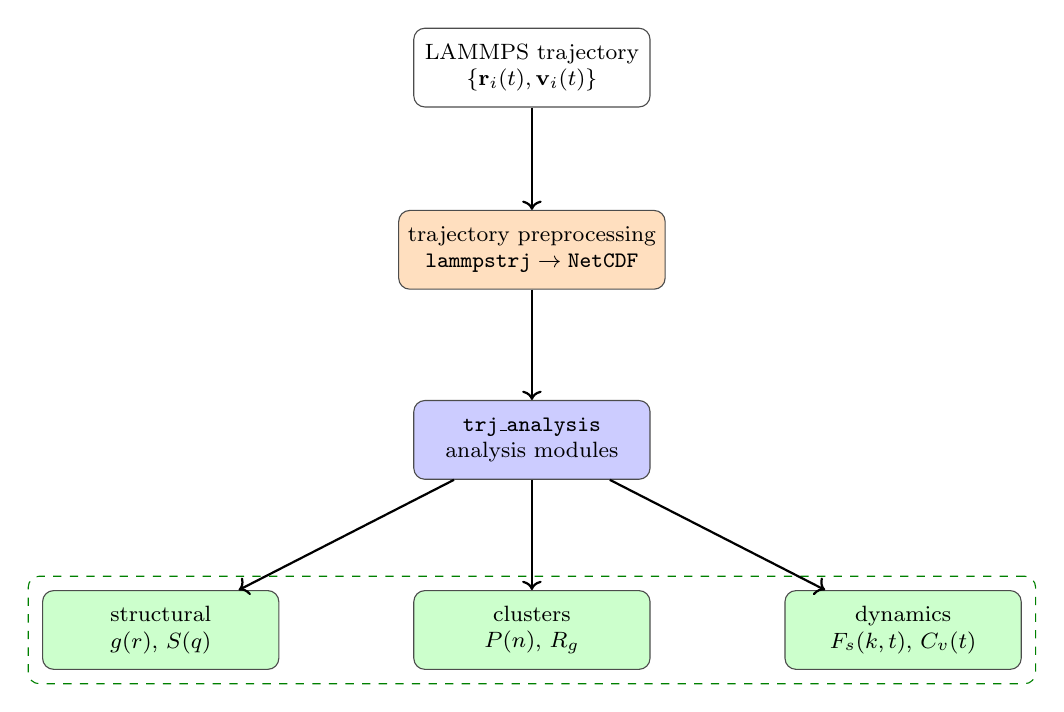
\begin{tikzpicture}[
box/.style={draw=black!70, rounded corners, align=center,
            minimum width=3cm, minimum height=1cm, font=\footnotesize},
tool/.style={box, fill=orange!25},
module/.style={box, fill=blue!20},
output/.style={box, fill=green!20},
group/.style={draw=green!50!black, dashed, rounded corners, inner sep=5pt},
arrow/.style={->, thick}
]

\node[box] (traj)
{LAMMPS trajectory\\$\{\mathbf r_i(t),\mathbf v_i(t)\}$};
\node[tool, below=1.3cm of traj] (tools)
{trajectory preprocessing\\$\texttt{lammpstrj}\rightarrow\texttt{NetCDF}$};

\node[module, below=1.4cm of tools] (analysis)
{\texttt{trj\_analysis}\\analysis modules};
\node[output, below left=1.4cm and 1.7cm of analysis] (struct)
{structural\\$g(r)$, $S(q)$};

\node[output, below=1.4cm of analysis] (cluster)
{clusters\\$P(n)$, $R_g$};
\node[output, below right=1.4cm and 1.7cm of analysis] (dyn)
{dynamics\\$F_s(k,t)$, $C_v(t)$};

\node[group, fit=(struct)(cluster)(dyn)] {};

\draw[arrow] (traj) -- (tools);
\draw[arrow] (tools) -- (analysis);
\draw[arrow] (analysis) -- (struct);
\draw[arrow] (analysis) -- (cluster);
\draw[arrow] (analysis) -- (dyn);
\end{tikzpicture}
\caption{Workflow of the \texttt{trj\_analysis} package.}
\label{fig:workflow}
\end{figure}


\section{Supported Observables}
 The current implementation includes the following analyses integrated in the codebase:

\subsection{Structural Analysis}

\subsubsection{Pair distribution functions}
The radial distribution function is defined as

\begin{equation}
g(r)=\frac{1}{4\pi r^2\rho N}
\left\langle \sum_{i,j}\delta(r-r_{ij}) \right\rangle ,
\end{equation}
For a system of $N$ particles in a volume $V$ with number density $\rho = N/V$, the discretized radial distribution function is computed as

\begin{equation}
g(r_k) = \frac{1}{N \rho \, 4\pi r_k^2 \Delta r}
\left\langle \sum_{i=1}^{N} \sum_{j \ne i}
\Theta(r_{ij} - r_k + \tfrac{\Delta r}{2})
\Theta(r_k + \tfrac{\Delta r}{2} - r_{ij})
\right\rangle ,
\end{equation}

where $r_{ij} = |\mathbf{r}_i - \mathbf{r}_j|$, $\Delta r$ is the bin width, and $\Theta$ is the Heaviside function. This translates into
\begin{equation}
g(r_k) = \frac{H(r_k)}{N \rho \, 4\pi r_k^2 \Delta r},
\end{equation}
where $H(r_k)$ is the histogram of pair distances. Our current
implementation makes use of tiling approaches to take advantage of
fast shared memory access in the GPU for the computation of the
particle-particle histograms following closely the strategy of Reuter
and Köfinger\cite{Reuter2019}. The code supports species-resolved
correlations $g_{\alpha\beta}(r)$ as well as explicit charge-charge
radial distribution functions $g_{qq}(r)$ if partial charges are
provided in the trajectory dump. Results are stored in {\tt
  gmixsim.dat}. Here it is worth to stress a particular feature of the
program's internal logic. For efficiency, LAMMPS atom types  are
remapped into contiguous internal IDs, {\tt 1\ldots nsp} (where {\tt
  nsp} is the number of atomic species), and then particle positions
are also remapped into the system memory once a simulation frame is
read, so as to keep all particles of the same species in contiguous
memory locations. This minimizes non-contiguous memory accesses when
computing species-resolved properties in mixtures. 


\subsubsection{Particle Number Fluctuations and Hyperuniformity}
In conjunction with the calculation of the radial distribution
functions, this code provides the possibility to characterize the
large-scale density fluctuations of  point patterns so as to assess
the presence of hyperuniformity\cite{Torquato2018a}. To that aim we analyze the
number variance $\sigma_N^2(R)$ within a spherical observation window
$\Omega$ of radius $R$. The number of particles $N(R)$ in the window
centered at position $\mathbf{x}_0$ is defined as:
\begin{equation}
N(R;\mathbf{x}_0) = \sum_{i=1}^{N} \chi_R(\mathbf{r}_i -
  \mathbf{x}_0)
\end{equation}
where $\chi_R(\mathbf{r})$ is the
indicator function of the window, which is 1 if $|\mathbf{r}| \le R$
and 0 otherwise. The local number variance is
then:
\begin{equation}
\sigma_N^2(R) = \langle N(R)^2 \rangle - \langle N(R) \rangle^2
\end{equation}
where $\langle \dots \rangle$ denotes an
ensemble average or an average over window centers
$\mathbf{x}_0$. This quantity is computed both for particles and for cluster centers
if the cluster analysis is enabled and the number of clusters is
larger that {\tt clthresh}. The number of sampling origins is
controlled by the input variable {\tt nrandom}. When this is set to
zero (default value) no fluctuation number analysis is carried out. 



\subsubsection{Static structure factors $S(q)$}

This quantity is defined as
  \begin{equation}
S(q)=\frac{1}{N}\langle \rho(\mathbf q)\rho(-\mathbf q)\rangle .
\end{equation}
  which once discretized reads
  \begin{equation}
S(\mathbf{q}) = \frac{1}{N}
\left\langle
\left| \sum_{j=1}^{N} e^{i \mathbf{q} \cdot \mathbf{r}_j} \right|^2
\right\rangle .
\end{equation}
Note that this quantity can also be computed from the Fourier
Transform of the radial distribution function. The direct evaluation
approach produces more accurate results for low-Q values, which would
otherwise be 
affected by truncation errors in $g(r)$. Additionally, finite-size
effects in $g(r)$ are known
to be more pronounced in the canonical ensemble than in the
grand-canonical ensemble, where particle-number fluctuations allow a
faster convergence towards the thermodynamic limit. In particular, the
pair distribution functions exhibit corrections of order $1/V$ in the
canonical ensemble, while grand-canonical estimates are generally
closer to their bulk values \cite{Lebowitz1961,Wang2017,Rogers2018}. 

Here the parallelization has been straightforward, with each GPU
thread being responsible to compute the contribution of each ${\bf
  Q}(ijk) = 2\pi(i/L_x,j/L_y,k/L_z)$, with $i,j,k =0,\ldots n_{max}$
and $L_m$ being the simulation cell dimension along the corresponding
$m$-axis. Note that the periodicity of the simulation box constraints
the values of the ${\bf Q}$ vector. The current program version only
gives meaningful structure factors (either static of dynamic) for
fully periodic samples. All contributions are added up in bins up to
{\tt qmin}, and from {\tt qmin} to {\tt qmax} only the Q-vectors
$2\pi(i/L_x,0,0)$, $2\pi(0,j/L_y,0)$, and $(0,0,k/L_z)$ are
averaged. Results for partial structure factors are stored in {\tt
  sqmix.dat}, and total structure factors in {\tt sq.dat}. 

\subsubsection{Confinement and Directional Profiles}
For systems under slit-pore confinement, the toolkit extracts highly localized structural information. While slit confinement calculations are internally evaluated using a canonical geometry with confining walls perpendicular to the $z$-axis, the user can designate any Cartesian direction ($x$, $y$, or $z$, corresponding to $\texttt{idir} = 1, 2, 3$) as the confinement axis in the trajectory file. When $\texttt{idir} \neq 3$, particle positions, velocities, forces, stress tensor components, and simulation cell parameters are automatically transposed upon trajectory reading into the internal reference frame, leaving downstream GPU kernels invariant.

Wall boundaries along the confinement axis are established according to the trajectory cell metadata:
\begin{itemize}
    \item When simulation box dimensions along the confinement axis are positive ($L_{\text{idir}} > 0$), particle coordinates are origin-shifted ($r - r_{\text{org}}$) and folded into $[0, L_{\text{idir}})$, setting wall positions at $[0, L_{\text{idir}}]$. This bypasses restrictions regarding non-zero origins in LAMMPS non-periodic boundary conventions.
    \item When box lengths are not explicitly defined in the trajectory ($L_{\text{idir}} = 0$), wall locations are determined adaptively from coordinate extremes augmented by a safety buffer ($p_{\text{wall}} = r_{\min} - 6\sigma$, $p_{\text{wall}}' = p_{\text{wall}} + L_{\text{eff}}$).
\end{itemize}

The module computes:
\begin{itemize}
    \item \textbf{Density Profiles:} 1D number density and charge
      density profiles computed across the confinement dimension ($\rho(z)$ and
      $\rho_q(z)$), normalized by the accessible pore volume. 
    \item \textbf{In-plane 2D Correlations:} Calculation of
      in-plane $g(r_{\perp})$ and $S(Q_{\perp})$ specifically evaluated within
      user-defined planar slices parallel to the confining walls. This
      includes species-resolved and charge-charge 2D correlations. 
\end{itemize}


\subsubsection{Bond orientational order parameters}

Bond orientational order parameters provide a quantitative measure of
the local structural organization of particles\cite{Steinhard1983} and
are widely used to identify crystalline, and  liquid-like cluster phases.

\begin{itemize}
\item {\bf 3D case. Steinhardt order parameters}
For each particle $i$, a set of complex coefficients is defined as
\begin{equation}
q_{lm}(i) = \frac{1}{N_b(i)} \sum_{j=1}^{N_b(i)}
Y_{lm}(\hat{\mathbf{r}}_{ij}),
\label{ylm}
\end{equation}
where $Y_{lm}$ are the spherical harmonics, $\hat{\mathbf{r}}_{ij}$ is the unit vector connecting particles $i$ and $j$, and $N_b(i)$ is the number of neighbors of particle $i$. The rotationally invariant bond order parameter is then defined as 
\begin{equation}
Q_l(i) = \left( \frac{4\pi}{2l+1}
\sum_{m=-l}^{l} |q_{lm}(i)|^2 \right)^{1/2}.
\end{equation}
A global order parameter can be obtained by averaging over all particles:
\begin{equation}
Q_l = \frac{1}{N} \sum_{i=1}^{N} Q_l(i).
\end{equation}
Typical choices are $l=4$ and $l=6$, which are sensitive to cubic and hexagonal symmetries, respectively.

\begin{algorithm}[H]
\caption{Cluster expansion (parallel BFS level)}
\label{alg:expand}
\begin{algorithmic}[1]
\Procedure{ExpandClusters}{labels, core\_flag, adj\_list, adj\_offsets}
\State labels$[\cdot]\leftarrow -1$, cluster\_id$\leftarrow 0$
\For{each unvisited core point $p$}
    \State labels$[p]\leftarrow$ cluster\_id
    \State frontier $\leftarrow \{p\}$
    \While{frontier $\neq \emptyset$}
        \State new\_frontier $\leftarrow \emptyset$ \Comment{parallel loop}
        \For{each $q$ in frontier \textbf{in parallel}}
            \State start $\leftarrow$ adj\_offsets[q], end $\leftarrow$ adj\_offsets[q+1]
            \For{$r$ in adj\_list[start:end]}
                \If{labels$[r]=-1$}
                    \State labels$[r]\leftarrow$ cluster\_id
                    \If{core\_flag[r]} \State new\_frontier $\leftarrow$ new\_frontier $\cup \{r\}$ \EndIf
                \EndIf
            \EndFor
        \EndFor
        \State frontier $\leftarrow$ new\_frontier
    \EndWhile
    \State cluster\_id$\leftarrow$ cluster\_id$+1$
\EndFor
\EndProcedure
\end{algorithmic}
\end{algorithm}


\item {\bf Two-dimensional bond order parameter}
For quasi-two-dimensional systems or planar structures, it is convenient to define a bond order parameter based on angular correlations\cite{Nelson1979}:
\begin{equation}
\phi_m(i) = \frac{1}{N_b(i)} \sum_{j=1}^{N_b(i)}
e^{i m \theta_{ij}},
\end{equation}
where $\theta_{ij}$ is the angle between the bond $\mathbf{r}_{ij}$ and a reference axis, and $m$ is an integer corresponding to the symmetry of interest (e.g., $m=6$ for hexagonal order). The magnitude of the order parameter is
\begin{equation}
|\phi_m(i)| = \left| \frac{1}{N_b(i)} \sum_{j=1}^{N_b(i)}
e^{i m \theta_{ij}} \right|.
\label{cossin}
\end{equation}
A global measure is obtained by averaging over all particles:
\begin{equation}
\phi_m = \frac{1}{N} \sum_{i=1}^{N} |\phi_m(i)|.
\end{equation}

\item{\bf Practical considerations and implementation}
The definition of neighbors $N_b(i)$ is crucial and is typically based
on a cutoff distance, $r_{cl}$ (which here is defined as the first
minimum of $g(r)$). Note that we will use this same separation as
connectivity distance when performing the cluster analysis. Now, the
parallelization will also be straightforward, each GPU thread being in
charge of the calculation of the corresponding order parameters for
each particle taking into account only the corresponding particle
neighbors, and then averaging over configurations and finally over all
particles. These last two operations are carried out on the CPU. The
algorithms implemented to evaluate both the spherical harmonics in
(\ref{ylm}) or the simpler $\sin m\phi, \cos m\phi$ functions in
(\ref{cossin}) resort to stable and numerically accurate recursion
formulae\cite{Winczewski2016}. Results are stored in {\tt order.dat}
and {\tt order\_per\_mol.dat}.  
\end{itemize}

\begin{figure}[t]
\centering
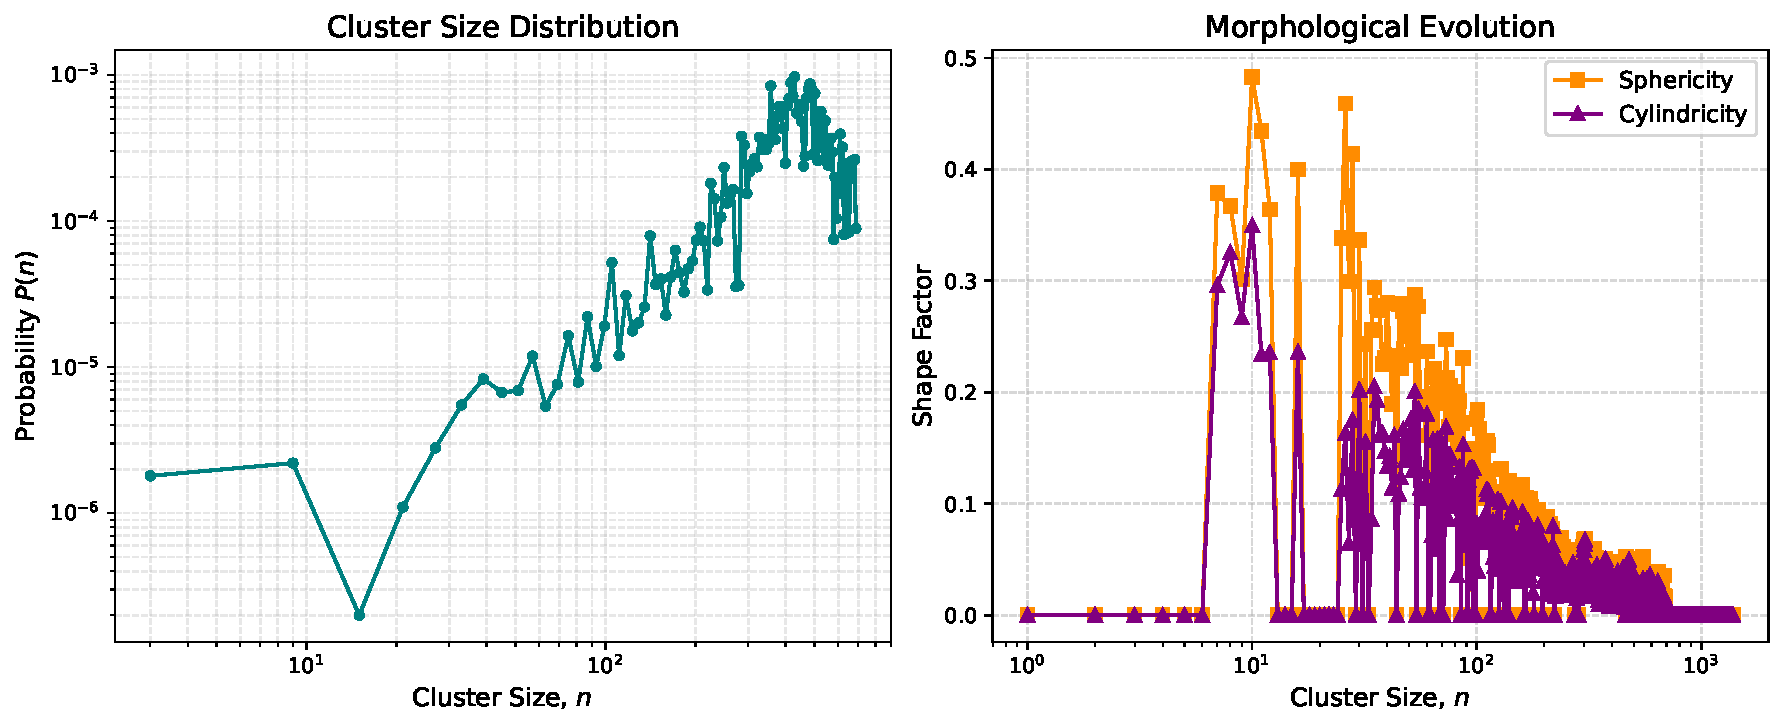
\includegraphics[width=\linewidth]{fig_morphology.pdf}
\caption{Evolution of cluster morphology for the 3D SALR system. Extracted from \texttt{fshape.dat} and \texttt{clustdistr.dat}, demonstrating the transition from globular to elongated structures as cluster size increases.}
\label{fig:morphology}
\end{figure}

\begin{figure}[t]
\centering
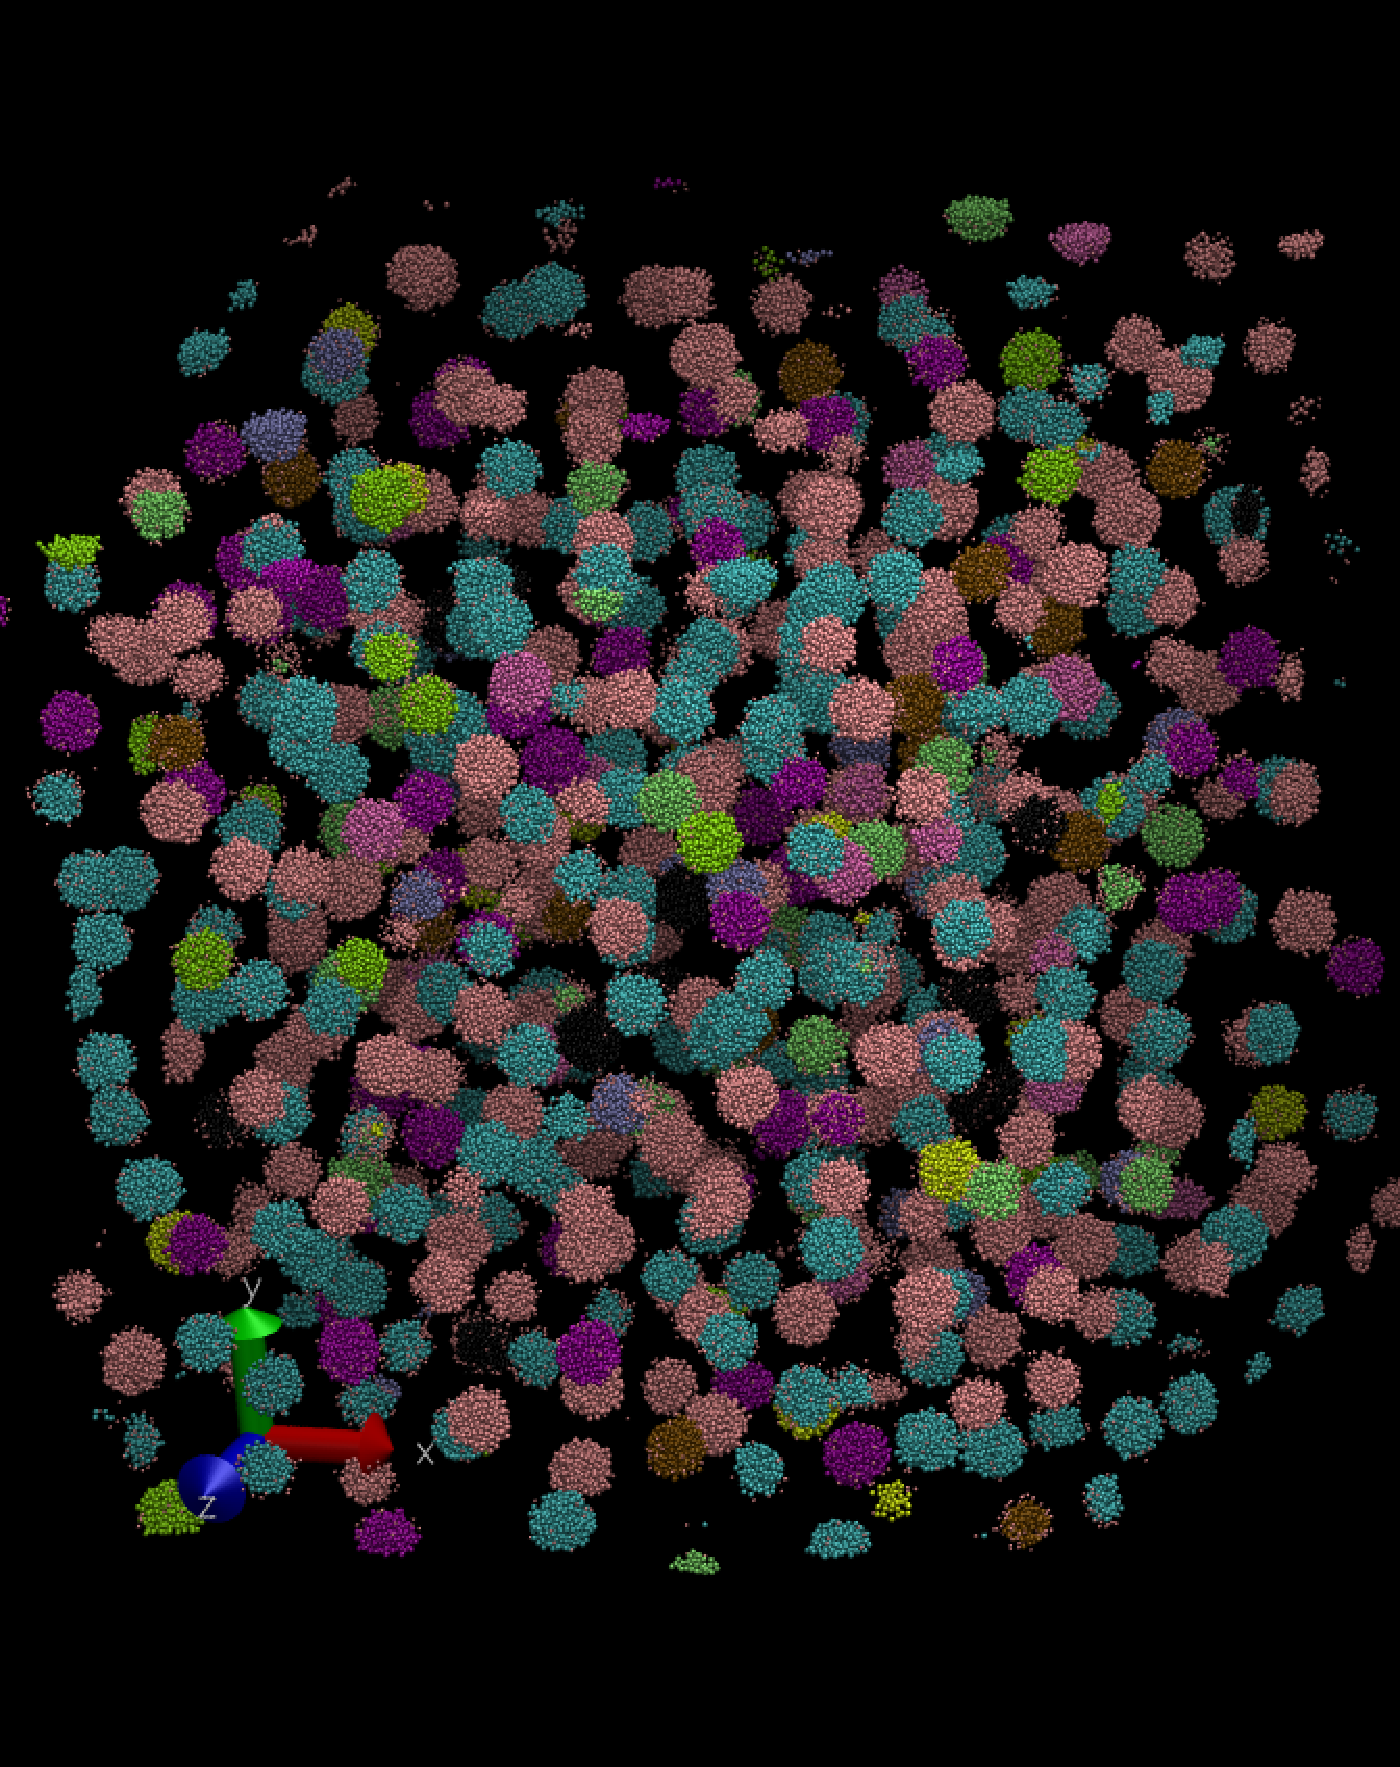
\includegraphics[width=0.6\linewidth]{fig_clusters.pdf}
\caption{Simulation snapshot of the 3D SALR system rendered using the generated \texttt{last\_clconf.lammpstrj}. Particles are colored by their \texttt{trj\_analysis} assigned cluster IDs.}
\label{fig:clusters}
\end{figure}


\subsection{Cluster Analysis}
This is one of the most time-consuming tasks when performing a configurational analysis in a purely serial code. When using neighbor lists the computational complexity is $O(N)$, and algorithms such as the density-based SCAN (DBSCAN) are particularly suited to a GPU implementation. Here we have followed the algorithm G-DBSCAN as developed by Andrade and coworkers\cite{Andrade2013}. In what follows we describe the key elements of our implementation.

\subsubsection{Neighbor list construction}
Here we use a linked cell approach\cite{AllenTildesleybook} in order to reduce the computational complexity of the neighbor search algorithm to $O(N)$. The linked cell list is computed in the CPU and transferred to the GPU devices. This could be further optimized by transferring the full computational load of the cell list to the GPU\cite{Schwiebert2014}, but the gain is negligible compared to other tasks, such as the Breadth-First-Search part\cite{Andrade2013} of the cluster construction. A single GPU thread is allocated to each particle and searches for its neighbors, marking all those with more than {\tt minPts -1} as {\em core} nodes, where {\tt minPts} is the minimum number of points (particles) to consider a cluster. Neighbors are stored in a one-dimensional adjacency list which is properly and efficiently organized using Thrust library parallel prefix sum (exclusive scan) operations\cite{ThrustDocumentation}.

\subsubsection{Cluster expansion}
Once the neighbor list is defined and nodes are identified as core or
border (connected but with less than {\tt minPts -1} neighbors),
clusters are expanded in a parallel Breadth-First-Search
fashion\cite{Andrade2013}. Each GPU thread starts from a core point,
and then each level processes border points, and adds unvisited
neighbors; the process is continued until no more new points are
left. All points connected to a core point are considered part of the
same cluster. Disconnected groups with less than {\tt minPts} points
are considered noise. The outer loop over clusters remains
sequential. The algorithm scheme, taken from
Ref.~\cite{LombaMoreno2026} is schematically shown in Algorithm
\ref{alg:expand}. 


Once clusters have been identified and classified in the corresponding
data structures the program determines the cluster size distribution
(basic minimum information provided), and if the number of clusters is
larger than {\tt clthresh} (defaults to 10) performs the following
analysis: 
\begin{itemize}
  \item Determine the distribution of gyration radii, defined as 
\begin{equation}
R_g = \left<\sqrt{\frac{\sum_i m_i ({\bf r}_i-{\bf R}_{com})^2}{\sum_i m_i}}\right>
\label{Rg}
\end{equation}
where $m_i$ and ${\bf r}_i$ are particle's mass and positions, and ${\bf R}_{com}$ is the clusters center of mass. Printout in {\tt radii.dat}.
  \item Cluster density profile, as calculated from the center of mass, stored in {\tt rhoprof.dat}, and the distribution of cluster internal densities, {\tt dens.dat}.
  \item If order parameters are calculated, in {\tt ordprof\_clust.dat} the corresponding spatial profiles of the order parameters, and their cumulative counterparts defined by 
\begin{equation}
Q_l^c(r) = \frac{3}{2r^3}\int_0^r {r'}^2Q_l(r') dr'.
\label{phi6c}
\end{equation}
are stored. 
\item Cluster-cluster correlations ($g_{cl-cl}$), inner cluster correlations ($g_{cl}$) and structure factors $S_{cl-cl}(Q)$ (in {\tt sqcl.dat}) are also calculated if requested.
\item Form factors quantifying the deviation from the spherical (or
  circular) shape and cylindrical shape are also determined and its
  distribution according to cluster size is stored in {\tt
    fshape.dat}. These quantities are computed from the values of the
  principal axes of inertia, after diagonalization of the inertia
  tensor (setting all masses to one, since we only care about the
  shape), and are defined by 
\begin{eqnarray}
f_{cyl} & = & \sqrt{\frac{|I_{yy}-I_{xx}|}{I_{xx}^2+I_{yy}^2+I_{zz}^2}}
  \\
f_{sph} & = & \sqrt{\frac{(I_{xx}-{\mbox\bf Tr}({\bf
              I}))^2+(I_{yy}-{\mbox\bf Tr}({\bf
              I}))^2}{I_{xx}^2+I_{yy}^2+I_{zz}^2}}
\end{eqnarray}
where ${\bf I}$ is the inertia matrix, $I_{zz}$ is its smallest
eigenvalue and $\mbox{\bf Tr}$ is the trace operator. If
$f_{cyl}\approx f_{sph}\rightarrow 0$ we have a spherical (circular)
shape. If only $f_{cyl}$ is significantly close to zero, we have a
cylindrical shape. 

\item Cluster center-of-mass trajectory output collected in {\tt centers.lammpstrj} using LAMMPS text dump format.
\item A LAMMPS dump file for the last configuration in which particle IDs are correlated to cluster sizes is also produced ({\tt last\_clconf.lammpstrj}) in addition of a direct dump of the last particle configuration as generated by LAMMPS ({\tt last\_conf.lammpstr}) for visualization purposes.
\end{itemize}

\subsection{Dynamical correlation functions}

Time-dependent observables are evaluated using multiple time origins in order to improve statistical accuracy. Given a trajectory sampled at discrete times
\[
t_n = n \Delta t, \quad n=0,\ldots,N_{\mathrm{conf}}-1,
\]
correlation functions are computed as averages over particles and time origins.

\subsubsection{Position self-correlation function}
The position self-correlation function is commonly expressed through the mean-square displacement (MSD):
\[
\mathrm{MSD}(t) = \left\langle \frac{1}{N} \sum_{i=1}^{N} \left| \mathbf{r}_i(t_0+t)-\mathbf{r}_i(t_0) \right|^2 \right\rangle_{t_0}.
\]
In discrete-time form, this becomes
\[
\mathrm{MSD}(m\Delta t)= \frac{1}{N(N_{\mathrm{conf}}-m)} \sum_{i=1}^{N} \sum_{n=0}^{N_{\mathrm{conf}}-m-1} \left| \mathbf{r}_i(t_{n+m})-\mathbf{r}_i(t_n) \right|^2.
\]
This estimator averages over all particles and available time origins.

\subsubsection{Velocity autocorrelation function}
The velocity autocorrelation function (VACF) is defined as
\[
C_v(t)= \left\langle \frac{1}{N} \sum_{i=1}^{N}
  \mathbf{v}_i(t_0+t)\cdot\mathbf{v}_i(t_0) \right\rangle_{t_0}. 
\]
Its discrete estimator reads
\[
C_v(m\Delta t)= \frac{1}{N(N_{\mathrm{conf}}-m)} \sum_{i=1}^{N}
\sum_{n=0}^{N_{\mathrm{conf}}-m-1} \mathbf{v}_i(t_{n+m})\cdot
\mathbf{v}_i(t_n). 
\]
The VACF provides access to transport coefficients such as the
diffusion constant via the Green--Kubo relation, and the corresponding
frequency spectrum, $Z(\omega)$, using a time resolved Fourier
transform, to which purpose we use here
the FFTW library\cite{Frigo2008FFTW3}. 

\subsubsection{Shear Viscosity from Green-Kubo Relations}

The shear viscosity
$\eta$, can be determined through the Green-Kubo formulation, which
relates the transport coefficient to the time-integral of the
auto-correlation function of its corresponding flux at equilibrium. 
In the limit of linear response theory, the shear viscosity $\eta$ is
given by the integral of the Stress Auto-Correlation Function (SACF): 

\begin{equation}
\eta = \frac{V}{k_B T} \int_0^\infty \langle P_{\alpha \beta}(t) P_{\alpha \beta}(0) \rangle dt
\end{equation}

where $k_B$ is the Boltzmann constant and $T$ is the absolute
temperature. For isotropic fluids, statistical accuracy is improved by
averaging over the three independent off-diagonal components: $P_{xy},
P_{xz},$ and $P_{yz}$. These quantities can be evaluated from the
forces, but here we have chosen to simply read in the corresponding
{\tt compute} (see \ref{therm} below) calculated by LAMMPS and stored
in the NetCDF dump file as a 
{\em per atom} quantity. 



As done for other dynamic correlations, in order  to maximize
statistical sampling from a finite trajectory of $N_T$ total steps, we
employ the method of multiple time origins. For a correlation lag time
$\tau = m \Delta t$, the discretized SACF, $C(m \Delta t)$, is
calculated as: 

\begin{equation}
C(m \Delta t) = \frac{1}{N(N_{\mathrm{conf}}-m)} \sum_{i=1}^{N} \sum_{n=0}^{N_{\mathrm{conf}}-m-1} P_{\alpha \beta}(t_k + m \Delta t) P_{\alpha \beta}(t_k)
\end{equation}
where $t_k$ represents the $k$-th time origin and $N_{orig}$ is the
total number of origins used.  Each CUDA thread will be in charge of
one time origin, the larger the number of origins the better the
statistics and the parallel performance of the code.  

The shear viscosity is then computed using a numerical integration
scheme, here the trapezoidal rule, up to a truncation time $M
\Delta t$ where the correlation has sufficiently decayed: 
\begin{equation}
\eta = \frac{V \Delta t}{k_B T} \left[ \frac{1}{2} C(0) + \sum_{m=1}^{M-1} C(m \Delta t) + \frac{1}{2} C(M \Delta t) \right]
\end{equation}
In practice, the choice of the maximum lag time $M \Delta t$ is
critical; it must be large enough to capture the decay of the SACF but
small enough to avoid the accumulation of statistical noise that
occurs at long times. 


\subsubsection{Self-intermediate scattering function}
The self part of the intermediate scattering function is defined as
\[
F_s(Q,t)= \left\langle \frac{1}{N} \sum_{i=1}^{N} e^{i\mathbf{Q}\cdot [\mathbf{r}_i(t_0+t)-\mathbf{r}_i(t_0)]} \right\rangle_{t_0}.
\]
Its discrete estimator becomes
\[
F_s(Q,m\Delta t)= \frac{1}{N(N_{\mathrm{conf}}-m)} \sum_{i=1}^{N} \sum_{n=0}^{N_{\mathrm{conf}}-m-1} e^{i\mathbf{Q}\cdot [\mathbf{r}_i(t_{n+m})-\mathbf{r}_i(t_n)]}.
\]
For isotropic systems, angular averaging over wavevectors of equal magnitude $Q=|\mathbf{Q}|$ is performed to improve statistics.

\subsubsection{Collective intermediate scattering function}
The collective intermediate scattering function is obtained from density fluctuations:
\[
F(Q,t)= \frac{1}{N} \left\langle \rho(\mathbf{Q},t_0+t) \rho(-\mathbf{Q},t_0) \right\rangle_{t_0},
\]
where
\[
\rho(\mathbf{Q},t)= \sum_{j=1}^{N} e^{i\mathbf{Q}\cdot\mathbf{r}_j(t)}.
\]
The corresponding discrete estimator reads
\[
F(Q,m\Delta t)= \frac{1}{N(N_{\mathrm{conf}}-m)} \sum_{n=0}^{N_{\mathrm{conf}}-m-1} \rho(\mathbf{Q},t_{n+m}) \rho(-\mathbf{Q},t_n).
\]

\subsubsection{Partial intermediate scattering functions}
For multicomponent systems, partial density functions are defined as
\[
\rho_\alpha(\mathbf{Q},t)= \sum_{j\in\alpha} e^{i\mathbf{Q}\cdot\mathbf{r}_j(t)},
\]
leading to
\[
F_{\alpha\beta}(Q,t)= \frac{1}{\sqrt{N_\alpha N_\beta}} \left\langle \rho_\alpha(\mathbf{Q},t_0+t) \rho_\beta(-\mathbf{Q},t_0) \right\rangle_{t_0}.
\]
These functions characterize cross-correlations between
species. Time-dependent observables are evaluated using a
multiple-time-origin buffering algorithm. This reduces the naive
quadratic scaling $\mathcal{O}(N_{\mathrm{conf}}^2)$ to approximately
$\mathcal{O}(N_{\mathrm{conf}} \log N_{\mathrm{conf}})$. These
quantities can be efficiently transformed to the frequency-domain
using again the FFTW library\cite{Frigo2008FFTW3}. In confined systems,
computation of the dynamical correlations $F(Q,t)$ and $S(Q,\omega)$
is automatically disabled. 

\subsection{Thermodynamic Quantities (if present in trajectory)\label{therm}}
If the LAMMPS NetCDF dump contains {\em per atom} quantities such as energy and/or pressure in addition to kinetic energy evaluation (when velocities are included in the dump), the code also computes:
\begin{itemize}
  \item Potential energy statistics per atom and per cluster if cluster analysis is also performed (generating {\tt distUcl\_N.dat} and {\tt distUcltot.dat}).
  \item Stress tensor and pressure evaluation. 
\end{itemize}
As mentioned, this requires LAMMPS to perform the appropriate {\tt computes} as follows:
\begin{lstlisting}[language=bash]
compute ener all pe/atom
compute stress all stress/atom NULL
dump trj1 all netcdf ${Ndump} run.nc id type x y z vx vy vz q c_stress[*] c_ener
\end{lstlisting}

\section{Installation and Usage}


\subsection{Requirements}
\begin{itemize}
  \item NetCDF library installation (Fortran and C interfaces), Fortran interface compiled with NVIDIA's \texttt{nvfortran}, \url{https://www.unidata.ucar.edu/software/netcdf}.
  \item FFTW3 library and development components. 
  \item Fortran compiler with F2008 support (e.g., \texttt{nvfortran}).
  \item C++ compiler (C++14 or newer, e.g., \texttt{nvcc}).
  \item NVIDIA HPC Software Development Kit (includes \texttt{nvfortran}), \url{https://developer.nvidia.com/hpc-sdk}
\end{itemize}

\subsection{Compilation}
Typical build commands:
\begin{lstlisting}[language=bash]
git clone https://github.com/elomba/trj_analysis
cd trj_analysis
# configure NetCDF, FFTW3, and CUDA paths
make
\end{lstlisting}
This will build a GPU-enabled program \texttt{trj\_analysis} in the
\texttt{trj\_analysis/bin}  directory.


\section{Program input description}

Input parameters are provided through Fortran namelists. Defaults are assigned internally whenever possible; otherwise parameters must be explicitly defined when activating the corresponding module. Some parameters inherit values from trajectory metadata and therefore become available only after the input file has been parsed. Unless otherwise specified, all lengths are expressed in simulation units.

\subsection{Global namelist: INPUT}
This namelist is mandatory.
\begin{center}
\begin{tabular}{llll}
\hline
Parameter & Type & Default & Notes \\
\hline
\texttt{trj\_input\_file} & string & required & NetCDF trajectory filename \\
\texttt{log\_output\_file} & string & analysis.log & Output log file \\
\texttt{ndim} & integer & 3 & Automatically overridden if detected in trajectory \\
\texttt{nsp} & integer & 1 & Updated after species detection if available \\
\texttt{ncfs\_from\_to} & integer(3) & 0,0,0 & Config range:
                                               [No. confs, start,
                                               end]. Default:  all \\
\texttt{rdf\_sq\_cl\_dyn\_sqw\_conf\_ord} & logical(7) & F,F,F,F,F,F,F & Module activation flags \\
\texttt{nthread} & integer & 64 & CUDA threads per block \\
\texttt{nqw} & integer & 0 & Used only if SQW module active \\
\texttt{nslice} & integer & 1 & Number of slices for confinement or profiling \\
\texttt{norder} & integer & 1 & Maximum order for Steinhardt parameters \\
\texttt{ener\_name} & string & none & Required only if energy histograms requested \\
\texttt{press\_name} & string & none & Required only if stress analysis requested \\
\texttt{potnbins} & integer & 100 & Energy histogram bins \\
\texttt{potengmargin} & real & 0.0 & Energy histogram margin \\
\texttt{rcl} & real & none & Required if clustering or order analysis active \\
\texttt{periodic} & logical array & T,T,T & Periodic boundary
                                            conditions per dimension
  \\
\texttt{topol} & logical & F & When true molecular topology is
                               analyzed\\
\texttt{system\_data\_file} & string & \texttt{system.data} & Topology
                                                           data file\\
\texttt{nprint} & integer & 10 & Printout frequency \\
\hline
\end{tabular}
\end{center}

\subsection{Species namelist: INPUT\_SP}
Required  for multicomponent/molecular systems or if the atomic mass
has to be specified. 
\begin{center}
\begin{tabular}{llll}
\hline
Parameter & Type & Default & Notes \\
\hline
\texttt{sp\_types\_selected} & integer array & 1 & LAMMPS type IDs for selected species \\
\texttt{mat} & real array & 1.0 & Atomic masses for each selected
                                  species \\
\texttt{rigid} & logical & F & If true rigid molecular units are present
  \\
\texttt{nmrigid} & integer & 0 & Number of types of rigid units \\
\texttt{rigid\_mols}& integer array & -- & IDs of rigid unit types \\
\hline
\end{tabular}
\end{center}

\subsection{Radial distribution functions: INPUT\_RDF}
Activated when RDF flag is true.
\begin{center}
\begin{tabular}{llll}
\hline
Parameter & Type & Default & Notes \\
\hline
\texttt{deltar} & real & 0.01 & Radial grid spacing \\
\texttt{rcrdf} & real & required & Must satisfy $r_{\mathrm{c}}<L/2$ \\
\texttt{nrandom} & integer & 0 & Number of random origins for fluctuation analysis \\
\hline
\end{tabular}
\end{center}

\subsection{Static structure factor: INPUT\_SQ}
Activated when SQ module enabled.
\begin{center}
\begin{tabular}{llll}
\hline
Parameter & Type & Default & Notes \\
\hline
\texttt{qmin} & real & required & Threshold for isotropic Q-sampling \\
\texttt{qmax} & real & required & Maximum Q value \\
\texttt{bsc} & real array & 1.0 & Coherent scattering lengths per species \\
\hline
\end{tabular}
\end{center}

\subsection{Cluster analysis: INPUT\_CL}
Activated when clustering flag is true.
\begin{center}
\begin{tabular}{llll}
\hline
Parameter & Type & Default & Notes \\
\hline
\texttt{dcl} & real & required & Grid spacing for cluster distributions \\
\texttt{minPts} & integer & $2\times\text{ndim}+1$ & Minimum cluster size \\
\texttt{ndrclus} & integer & 1 & Bins for cluster radial profiles \\
\texttt{cl\_thresh} & integer & 10 & Minimum cluster count for correlations \\
\texttt{geometry} & logical & T & Enables geometry and shape computations \\
\hline
\end{tabular}
\end{center}

\subsection{Confinement analysis: INPUT\_CONF}
Activated when confinement flag enabled.
\begin{center}
\begin{tabular}{llll}
\hline
Parameter & Type & Default & Notes \\
\hline
\texttt{idir} & integer & 3 & Confinement axis in trajectory (1=$x$, 2=$y$, 3=$z$) \\
\texttt{zslice} & real array & none & Explicit slice positions along the confinement axis \\
\texttt{zgrid} & real & none & Grid spacing / slice thickness for profiles \\
\hline
\end{tabular}
\end{center}

\subsection{Dynamical correlations: INPUT\_DYN}
Activated when dynamical module enabled.
\begin{center}
\begin{tabular}{llll}
\hline
Parameter & Type & Default & Notes \\
\hline
\texttt{nbuffer} & integer & 2 & Number of time origins for correlation \\
\texttt{tmax} & real & -1.0 & Max time window for correlations (ps) \\
\texttt{tmaxp} & real & -1.0 & Max time for viscosity windowing \\
\texttt{tlimit} & real & -1.0 & Global time limit for buffer averaging \\
\texttt{jump} & integer & 1 & Config stride between buffers \\
\hline
\end{tabular}
\end{center}

\subsection{Dynamic structure factor: INPUT\_SQW}
Activated when SQW module enabled.
\begin{center}
\begin{tabular}{llll}
\hline
Parameter & Type & Default & Notes \\
\hline
\texttt{qw} & real array & required & Q-values for $F(Q,t)$ and $S(Q,\omega)$ \\
\texttt{tmqw} & real array & required & Maximum times per specific Q-value \\
\hline
\end{tabular}
\end{center}

\subsection{Bond–orientational order: INPUT\_ORDER}
Activated when order-analysis flag enabled.
\begin{center}
\begin{tabular}{llll}
\hline
Parameter & Type & Default & Notes \\
\hline
\texttt{orderp} & integer array & required & Harmonic indices $\ell$ for Steinhardt parameters \\
\texttt{print\_orderp} & logical & F & Enables per-particle output \\
\texttt{nnbond} & integer & 0 & Fixed neighbor count (0 = use cutoff \texttt{rcl}) \\
\texttt{rclcl} & real & 0.0 & Cutoff for inter-cluster neighbors \\
\hline
\end{tabular}
\end{center}

\subsection{Implicit and trajectory-derived defaults}
Some parameters are determined automatically after reading trajectory metadata:
\begin{itemize}
\item number of configurations $N_{\mathrm{conf}}$
\item simulation box dimensions
\item particle number $N$
\item species populations $N_\alpha$
\item dimensionality (if stored in trajectory)
\item accessible correlation time window
\end{itemize}
These quantities override user defaults when present. 


\section{Output files}

Table~\ref{tab:trj_output_files} lists the output files generated by \texttt{trj\_analysis}. Files are produced only when the corresponding analysis modules are activated.

\begin{table*}[htbp]
\centering
\caption{Output files generated by \texttt{trj\_analysis}.}
\label{tab:trj_output_files}
\begin{tabular}{lll}
\toprule
File name & Observable & Conditions \\
\midrule
\multicolumn{3}{c}{\textit{Thermodynamics \& General Output}} \\
\midrule
\texttt{analysis.log} & Execution log and parameter summary & Always written \\
\texttt{thermo\_run.dat} & Time series of instantaneous $T$, $P$, and
                           internal energy & if $P$, and $U$ in dump \\
\texttt{pot\_energy.dat} & Global per-atom potential energy distributions & \texttt{ener\_name} defined \\
\midrule
\multicolumn{3}{c}{\textit{Structural Analysis}} \\
\midrule
\texttt{gmixsim.dat} & Pair distribution functions $g_{\alpha\beta}(r)$ & RDF module active \\
\texttt{s2n.dat} & Number fluctuation data & \texttt{nrandom} $> 0$ \\
\texttt{sq.dat} & Total static structure factor $S(Q)$, $S_{NN}(Q)$, $S_{cc}(Q)$ & SQ module active \\
\texttt{sqmix.dat} & Species-resolved partial structure factors & SQ module active \\
\texttt{sqcl.dat} & Cluster-center structure factor $S_{cl}(Q)$ & CL + SQ modules \\
\texttt{order.dat} & Averaged Steinhardt order parameters $\langle Q_l \rangle$ & ORDER module active \\
\texttt{order\_per\_mol.dat} & Per-particle order parameters & \texttt{print\_orderp} = T \\
\midrule
\multicolumn{3}{c}{\textit{Directional \& Confinement Analysis}} \\
\midrule
\texttt{densprof.dat} & Density profile along the confinement axis (\texttt{idir}) & CONF module active \\
\texttt{qdens.dat} & Total and species-resolved charge density profiles & CONF + charges present \\
\texttt{gxy\_i-j.dat} & In-plane 2D RDFs calculated within slices parallel to walls & CONF + RDF \\
\texttt{gxy\_qq.dat} & In-plane 2D charge-charge RDF within slices parallel to walls & CONF + RDF + charges \\
\texttt{sqxy.dat} & In-plane 2D structure factor calculated within slices parallel to walls & CONF + SQ \\
\texttt{sqxy\_qq.dat} & In-plane 2D charge-charge structure factor within slices parallel to walls & CONF + SQ + charges \\
\texttt{sqpxy\_i-i.dat} & In-plane partial 2D structure factors per species within slices & CONF + SQ \\
\midrule
\multicolumn{3}{c}{\textit{Cluster Analysis}} \\
\midrule
\texttt{clustdistr.dat} & Cluster size distribution & CL module active \\
\texttt{radii.dat} & Distribution of cluster radii of gyration & CL module active \\
\texttt{rhoprof.dat} & Average cluster radial density profiles & CL module active \\
\texttt{fshape.dat} & Cluster shape descriptors (sphericity, cylindricity) & \texttt{geometry} = T \\
\texttt{distUcl\_N.dat} & Distribution of internal energy per particle & CL + \texttt{ener\_name} \\
\texttt{distUcltot.dat} & Distribution of total cluster internal energy & CL + \texttt{ener\_name} \\
\texttt{clusevol.dat} & Time evolution of cluster counts and clustered fractions & CL module active \\
\texttt{order\_per\_clust.dat}& Order parameters averaged per cluster & CL + ORDER \\
\texttt{ordprof\_clust.dat} & Steinhardt parameter profiles across cluster slices & CL + ORDER \\
\texttt{ordprof\_clcum.dat} & Cumulative Steinhardt profiles & CL + ORDER \\
\texttt{centers.lammpstrj} & Cluster center-of-mass trajectory for visualization & CL module active \\
\texttt{last\_clconf.lammpstrj}& Final configuration with particles colored by cluster ID & CL module active \\
\midrule
\multicolumn{3}{c}{\textit{Dynamical Correlations}} \\
\midrule
\texttt{dyn.dat} & Mean squared displacement and velocity autocorrelation & DYN module active \\
\texttt{dynw.dat} & Frequency-resolved impedance $Z(\omega)$ & DYN module active \\
\texttt{fkt.dat} & Coherent intermediate scattering function $F(Q,t)$ & SQW module active \\
\texttt{fskt.dat} & Self-intermediate scattering function $F_s(Q,t)$ & SQW module active \\
\texttt{sqw.dat} & Dynamic structure factors $S(Q,\omega)$ and $S_s(Q,\omega)$ & SQW module active \\
\texttt{viscor.dat} & Stress autocorrelation and shear viscosity $\eta(t)$ & DYN + \texttt{press\_name} \\
\bottomrule
\end{tabular}
\end{table*}

\begin{figure}[t]
\centering
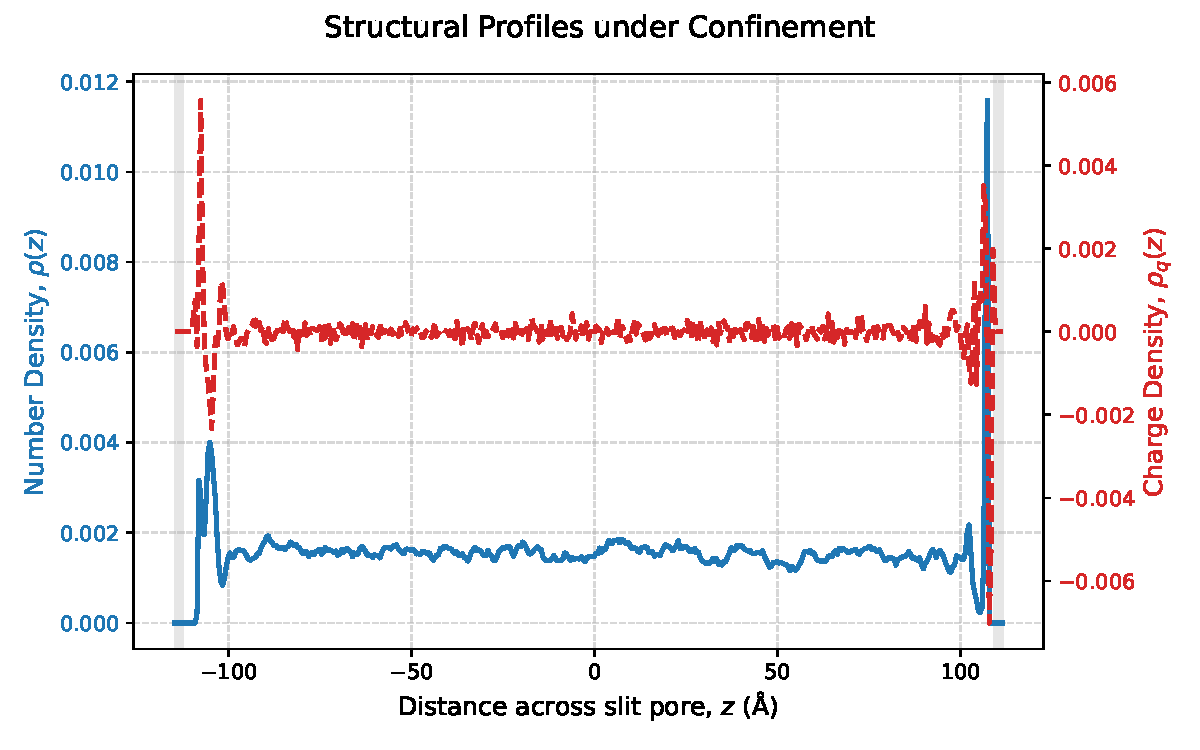
\includegraphics[width=\linewidth]{fig_confinement.pdf}
\caption{Density $\rho(z)$ and charge density $\rho_q(z)$ profiles for an ionic liquid confined between charged plates, extracted from \texttt{densprof.dat} and \texttt{qdens.dat} using the \texttt{CONF} module.}
\label{fig:confinement}
\end{figure}

\begin{figure}[t]
\centering
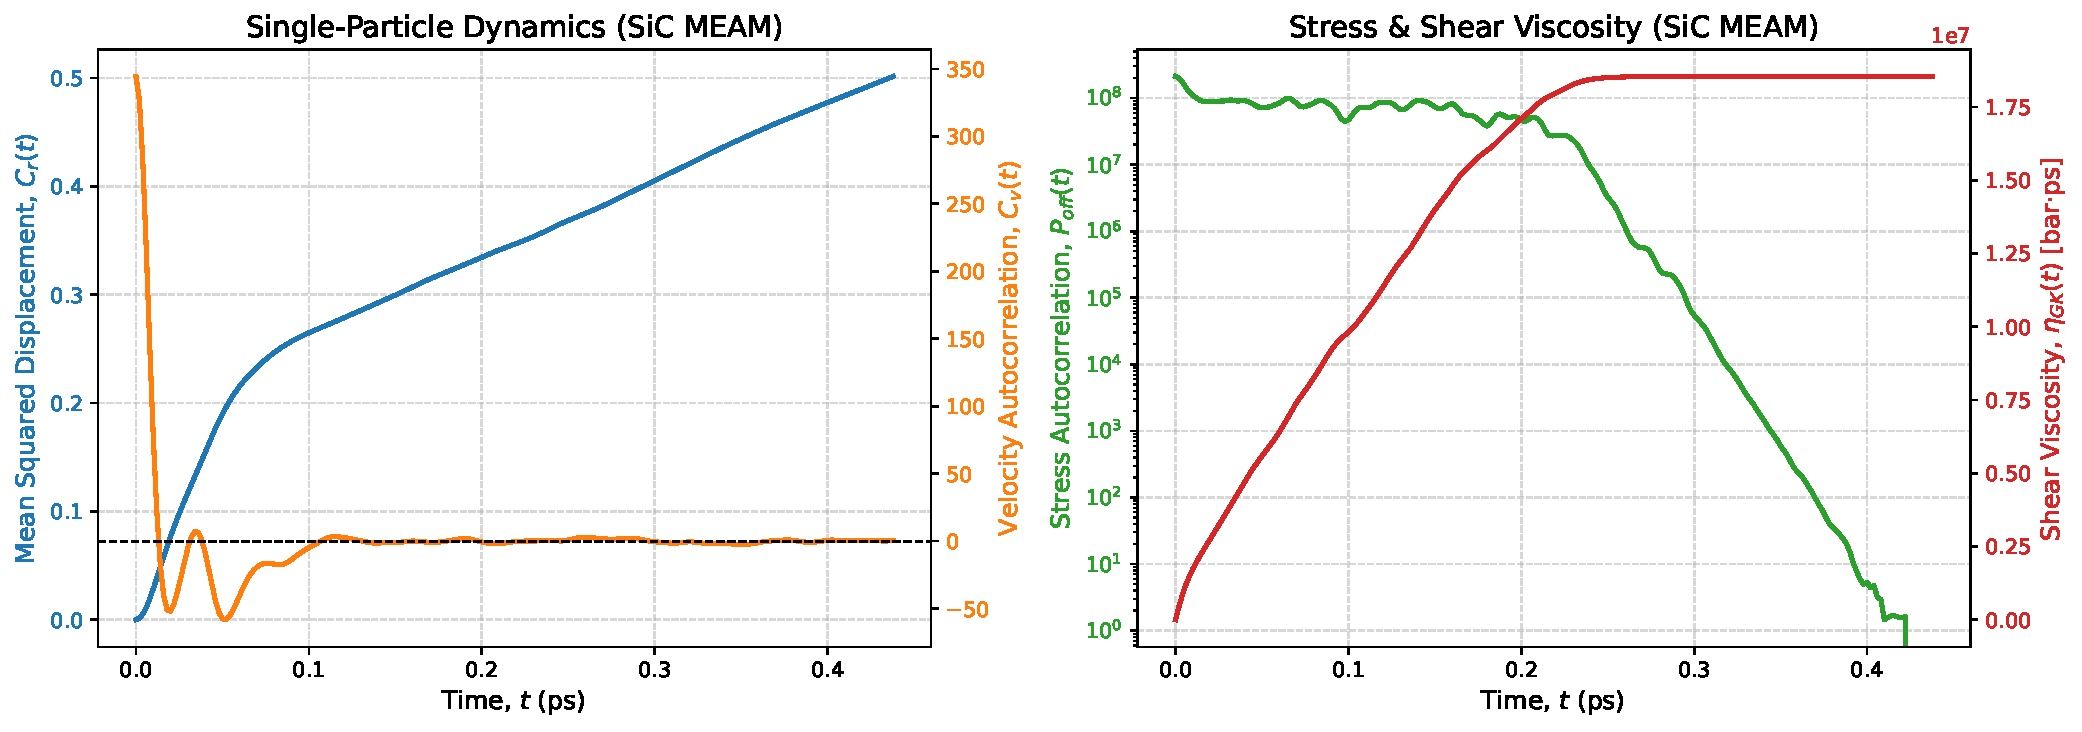
\includegraphics[width=\linewidth]{fig_dynamics.pdf}
\caption{Dynamical properties and transport coefficients for a silicon carbide (SiC) alloy modeled with a MEAM potential. (Left) Single-particle dynamics showing the mean squared displacement (MSD) and the highly oscillatory velocity autocorrelation function (VACF) typical of solid-state phonon dynamics, evaluated using the multi-origin buffering algorithm and extracted from \texttt{dyn.dat}. (Right) Collective dynamics illustrating the rapid decay of the off-diagonal stress autocorrelation function (SACF) alongside the convergence of the running integral for the Green-Kubo shear viscosity ($\eta_{GK}$), extracted from \texttt{viscor.dat}.}
\label{fig:dynamics}
\end{figure}

\section{Example Usage and validation}

An example run on a NetCDF trajectory file:
\begin{lstlisting}[language=bash]
./trj_analysis input.nml GPU_id
\end{lstlisting}
where \texttt{GPU\_id} is the number identifying a GPU device (as given by \texttt{nvidia-smi}), and \texttt{input.nml} is a file containing the namelists specified above.


The correctness of observables was verified using a variety of canonical MD test
systems. For structural observables like pair distribution functions
and static structure factors, comparisons to reference calculations
showed agreement within statistical uncertainties. Dynamical
observables such as time correlation functions and MSDs similarly
matched expected behavior.  

A comprehensive set of validation examples is included in the
repository under the directory \texttt{examples/} (cf tree of Figure
\ref{fig:repo_structure}). The examples cover several types of systems
commonly encountered in soft-matter and molecular simulations. Also to
showcase the capabilities of the toolkit, we have extracted data from
the provided validation examples and generated representative figures
for some of the examples cited below. 

\begin{itemize}
\item SALR systems (short-range attraction / long-range repulsion)
  exhibiting cluster formation, both in 3D and 2D. These examples are
  taken from Refs. \cite{DiazPozuelo202y5} and \cite{Bores2026}
  respectively. In Figure \ref{fig:morphology} we observe the size
  distribution of a system of 3D SALR clusters (left) and the
  distribution of shape factors (right). The distribution indicates a
  dominance of large spherical clusters, with important deviations
  for small sizes. A snapshot that illustrates the clusters is
  presented in Figure \ref{fig:clusters}.

\item A simple binary Lennard-Jones mixture in which LAMMPS {\tt lj}-units are used.


\item A coarse grained model of ionic liquid and TIP4p/2005 water
  between two plates at constant potential taken from
  \cite{Lomba2024}. The corresponding number and charge density
  profiles is plotted in Figure \ref{fig:confinement}. The marked
  charge asymmetry induced by the potential difference is clearly
  visible. 

\item The dynamics of a molten SiC alloy described using a MEAM potential
  \cite{Baskes1992} was also analyzed and in Figure
  \ref{fig:dynamics} we can see the behavior of the mean square
  displacement and velocity autocorrelation (left), and stress
  autocorrelation and shear viscosity (right). The curves display a good
  convergence that results from the  use of 40 time origins, separated by 20
  stored configurations (2 ps). {\tt metal} units are used.

\end{itemize}


\begin{table}[htbp]
\centering
\caption{Benchmark comparison between CPU and GPU implementations for structural analysis calculations.\label{bench}}
\begin{tabular}{lcccccc}
\toprule
& \multicolumn{3}{c}{97,336 particles} & \multicolumn{3}{c}{216,000 particles} \\ \midrule

Method & CPU (s) & GPU (s) & Speedup & CPU (s) & GPU (s) & Speedup \\
\midrule
$g(r)$ & 8.40 & 0.03 & 280$\times$ & 17.40 & 0.165 & 105$\times$ \\
$Q_4, Q_6, Q_8, Q_{10}, Q_{12}$ & 0.02 & 0.003 & 6.7$\times$ & 0.17 & 0.008 & 21$\times$ \\
$S(Q)$ & 4.45 & 0.09 & 49$\times$ & 22.00 & 0.29 & 76$\times$ \\
Cluster analysis & 26.6 & 0.12 & 220$\times$ & 64.00 & 0.25 & 250$\times$ \\
\bottomrule
\end{tabular}
\end{table}





\section{Performance}

Performance was benchmarked using an Intel Xeon Gold 6548Y+ dual
processor and an NVIDIA RTX Pro 4500 Blackwell with Compute Capability
12.0. In Table \ref{bench} we present a comparison for various
structural properties and cluster analysis. For the calculation of the
pair distribution function and orientational bond order
parameters\cite{Steinhard1983} LAMMPS built-in {\tt compute rdf} and
{\tt compute orientorder/bond} were employed by means of  a {\tt
  rerun} over a stored trajectory. This allows
the calculation of $g(r)$ values beyond the potential cutoff and does
not include the computational cost of the simulation itsel. Moreover,
I/O time was also subtracted from the total CPU time. The
corresponding LAMMPS scripts are collected in the {\tt tools/}
directory. The
static structure factor was computed using the script {\tt
  fast\_sq\_freud\_netcdf.py} included in the directory {\tt
  tools/}. This script uses a optimized routine for direct structure
factor evaluation from Freud 3.5.0 package\cite{freud2020}, {\tt
  freud.diffraction.StaticStructureFactorDirect}. From the
table it is evident that GPU acceleration yields a very significant
reductions in runtime for histogram and correlation tasks compared to
CPU-only routines, allowing analysis of large trajectories in
practical wall-clock times. Speed-up for dynamic correlations are not
included, since in this version parallelization is only implemented at
the level of multiple time-origin selection, and results are
comparable to optimized approaches such as the Fast Correlation
Analysis using Fast Fourier Transforms\cite{Kneller1995FCA}. A GPU
version of this approach will be incorporated in a future release.
Finally, the CPU analysis of clusters was carried out implementing a
DBSCAN algorithm in a highly optimized code that uses NUMBA libraries
\cite{Lamaetal2015,LombaMoreno2026}. 

\begin{sidewaysfigure}[htbp]
\centering
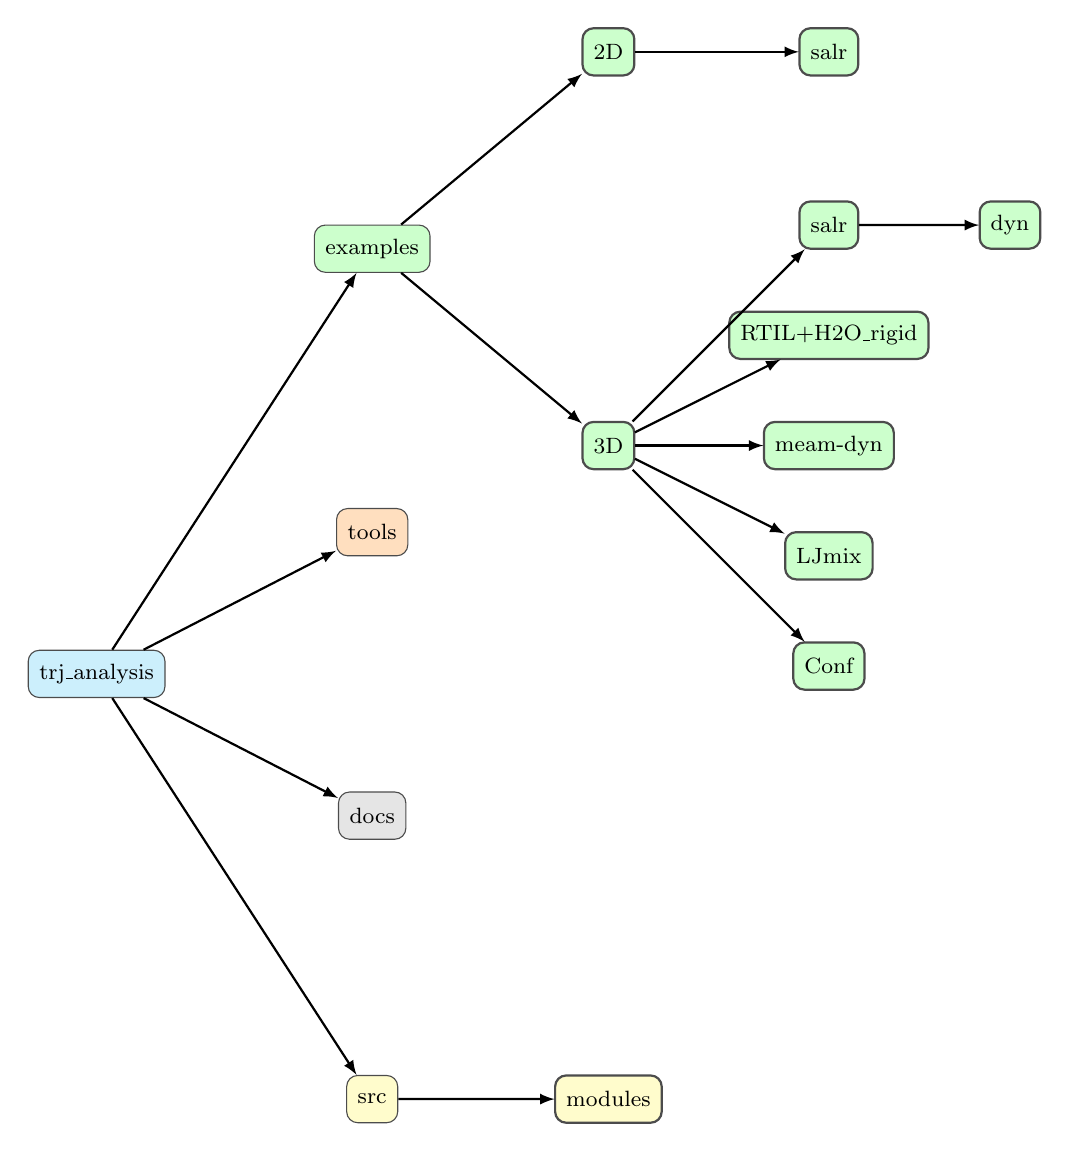
\begin{tikzpicture}[
  grow=right,
  edge from parent/.style={draw, -latex, thick},
  node/.style={draw=black!70, rounded corners, align=center, font=\footnotesize, minimum height=0.6cm, inner sep=4pt},
  dir/.style={node, fill=cyan!20},
  src/.style={node, fill=yellow!20},
  ex/.style={node, fill=green!20},
  tool/.style={node, fill=orange!25},
  doc/.style={node, fill=gray!20},
  % -- ADJUSTED SPACING --
  level 1/.style={sibling distance=3.6cm, level distance=3.5cm},
  % Increased from 2.4cm to 5.0cm to separate the 3D and 2D subtrees
  level 2/.style={sibling distance=5.0cm, level distance=3.0cm},
  % Increased sibling distance from 1.1cm to 1.4cm so the 5 nodes don't touch
  % Increased level distance slightly to 2.8cm to account for the wide "RTIL+H2O_rigid" text
  level 3/.style={sibling distance=1.4cm, level distance=2.8cm},
  level 4/.style={sibling distance=1.1cm, level distance=2.3cm}
]

\node[dir] {trj\_analysis}
  child { node[src] {src}
    child { node[src] {modules} }
        }
  child { node[doc] {docs} }
  child { node[tool] {tools} }
  child { node[ex] {examples}
    child { node[ex] {3D}
      child { node[ex] {Conf} }
      child { node[ex] {LJmix} }
      child { node[ex] {meam-dyn} }
      child { node[ex] {RTIL+H2O\_rigid} }
      child { node[ex] {salr}
        child { node[ex] {dyn} }
      }
    }
    child { node[ex] {2D}
      child { node[ex] {salr} }
    }
  };

\end{tikzpicture}
\caption{Directory structure of the \texttt{trj\_analysis} repository. The software is organized into modules for structural, clustering, order-parameter and dynamical analysis. Example workflows and trajectory utilities are provided in the \texttt{examples/} and \texttt{tools/} directories.}
\label{fig:repo_structure}
\end{sidewaysfigure}



\section{Availability and Documentation}

The code for \texttt{trj\_analysis} is available at:
\begin{center}
\url{https://github.com/elomba/trj_analysis}
\end{center}

The repository includes example input files, output examples,
documentation, and validation cases to facilitate usage and extension,
all organized as indicated in the diagram of Figure
\ref{fig:repo_structure}. Both the parent directory, {\tt tools/} and
{\tt examples/} directories include the corresponding {\tt README.md}
files explaining the contents and basic instructions. 

\section{Conclusions}

\texttt{trj\_analysis} provides a scalable, GPU-accelerated toolkit
for analyzing LAMMPS NetCDF trajectories. The combination of Fortran,
C++, and GPU support enables efficient processing for large systems
and long trajectories yielding a large panoply of physical
quantities. The modular structure supports extensibility 
for new observables and workflows. Future releases will include an
improved computation of dynamic correlations, and an extended tool
library for the topological analysis of complex cluster structures. 

\section{Declaration of generative AI and AI-assisted technologies in
  the manuscript preparation process} 

During the preparation of this work the authors used Gemini 3.1 in
order to generate input parameter and output file tables and
flow/directory structure diagrams. After using this tool, the authors
reviewed and edited the content as needed and takes full
responsibility for the content of the published article. 

\section*{Acknowledgements}

EL and ADP acknowledge the financial support from Grant No. PID2023-151751NB-I00 funded by MICIU/AEI/10.13039/501100011033 and by ``ERDF A way of making Europe.'' We would also like to acknowledge the Galicia Supercomputing Center (CESGA) for the generous access to their computer facilities.

% ======================================================================
% Bibliography
% ======================================================================
\bibliographystyle{elsarticle-num}
\bibliography{refs}

\end{document}
